%%
% Copyright (c) 2017 - 2019, Pascal Wagler;  
% Copyright (c) 2014 - 2019, John MacFarlane
% 
% All rights reserved.
% 
% Redistribution and use in source and binary forms, with or without 
% modification, are permitted provided that the following conditions 
% are met:
% 
% - Redistributions of source code must retain the above copyright 
% notice, this list of conditions and the following disclaimer.
% 
% - Redistributions in binary form must reproduce the above copyright 
% notice, this list of conditions and the following disclaimer in the 
% documentation and/or other materials provided with the distribution.
% 
% - Neither the name of John MacFarlane nor the names of other 
% contributors may be used to endorse or promote products derived 
% from this software without specific prior written permission.
% 
% THIS SOFTWARE IS PROVIDED BY THE COPYRIGHT HOLDERS AND CONTRIBUTORS 
% "AS IS" AND ANY EXPRESS OR IMPLIED WARRANTIES, INCLUDING, BUT NOT 
% LIMITED TO, THE IMPLIED WARRANTIES OF MERCHANTABILITY AND FITNESS 
% FOR A PARTICULAR PURPOSE ARE DISCLAIMED. IN NO EVENT SHALL THE 
% COPYRIGHT OWNER OR CONTRIBUTORS BE LIABLE FOR ANY DIRECT, INDIRECT, 
% INCIDENTAL, SPECIAL, EXEMPLARY, OR CONSEQUENTIAL DAMAGES (INCLUDING,
% BUT NOT LIMITED TO, PROCUREMENT OF SUBSTITUTE GOODS OR SERVICES; 
% LOSS OF USE, DATA, OR PROFITS; OR BUSINESS INTERRUPTION) HOWEVER 
% CAUSED AND ON ANY THEORY OF LIABILITY, WHETHER IN CONTRACT, STRICT 
% LIABILITY, OR TORT (INCLUDING NEGLIGENCE OR OTHERWISE) ARISING IN 
% ANY WAY OUT OF THE USE OF THIS SOFTWARE, EVEN IF ADVISED OF THE 
% POSSIBILITY OF SUCH DAMAGE.
%%

%%
% This is the Eisvogel pandoc LaTeX template.
%
% For usage information and examples visit the official GitHub page:
% https://github.com/Wandmalfarbe/pandoc-latex-template
%%

\PassOptionsToPackage{unicode=true}{hyperref} % options for packages loaded elsewhere
\PassOptionsToPackage{hyphens}{url}
\PassOptionsToPackage{dvipsnames,svgnames*,x11names*,table}{xcolor}
%
\documentclass[
  10pt,
  english,
  letterpaper,
,tablecaptionabove
]{scrartcl}
\usepackage{lmodern}
\usepackage{setspace}
\setstretch{1.2}
\usepackage{amssymb,amsmath}
\usepackage{ifxetex,ifluatex}
\ifnum 0\ifxetex 1\fi\ifluatex 1\fi=0 % if pdftex
  \usepackage[T1]{fontenc}
  \usepackage[utf8]{inputenc}
  \usepackage{textcomp} % provides euro and other symbols
\else % if luatex or xelatex
  \usepackage{unicode-math}
  \defaultfontfeatures{Scale=MatchLowercase}
  \defaultfontfeatures[\rmfamily]{Ligatures=TeX,Scale=1}
\fi
% use upquote if available, for straight quotes in verbatim environments
\IfFileExists{upquote.sty}{\usepackage{upquote}}{}
\IfFileExists{microtype.sty}{% use microtype if available
  \usepackage[]{microtype}
  \UseMicrotypeSet[protrusion]{basicmath} % disable protrusion for tt fonts
}{}
\makeatletter
\@ifundefined{KOMAClassName}{% if non-KOMA class
  \IfFileExists{parskip.sty}{%
    \usepackage{parskip}
  }{% else
    \setlength{\parindent}{0pt}
    \setlength{\parskip}{6pt plus 2pt minus 1pt}}
}{% if KOMA class
  \KOMAoptions{parskip=half}}
\makeatother
\usepackage{xcolor}
\definecolor{default-linkcolor}{HTML}{A50000}
\definecolor{default-filecolor}{HTML}{A50000}
\definecolor{default-citecolor}{HTML}{4077C0}
\definecolor{default-urlcolor}{HTML}{4077C0}
\IfFileExists{xurl.sty}{\usepackage{xurl}}{} % add URL line breaks if available
\IfFileExists{bookmark.sty}{\usepackage{bookmark}}{\usepackage{hyperref}}
\hypersetup{
  pdftitle={Disjoint Sets and Union Find},
  pdfauthor={Connor Baker},
  pdfsubject={Disjoint Sets and Union Find},
  pdfkeywords={Lecture, Disjoint Sets, Union Find},
  pdfborder={0 0 0},
  breaklinks=true}
\urlstyle{same}  % don't use monospace font for urls
\usepackage[margin=2.5cm,includehead=true,includefoot=true,centering]{geometry}
\usepackage{listings}
\newcommand{\passthrough}[1]{#1}
\lstset{defaultdialect=[5.3]Lua}
\lstset{defaultdialect=[x86masm]Assembler}
\usepackage{longtable,booktabs}
% Allow footnotes in longtable head/foot
\IfFileExists{footnotehyper.sty}{\usepackage{footnotehyper}}{\usepackage{footnote}}
\makesavenoteenv{longtable}
\usepackage{graphicx,grffile}
\makeatletter
\def\maxwidth{\ifdim\Gin@nat@width>\linewidth\linewidth\else\Gin@nat@width\fi}
\def\maxheight{\ifdim\Gin@nat@height>\textheight\textheight\else\Gin@nat@height\fi}
\makeatother
% Scale images if necessary, so that they will not overflow the page
% margins by default, and it is still possible to overwrite the defaults
% using explicit options in \includegraphics[width, height, ...]{}
\setkeys{Gin}{width=\maxwidth,height=\maxheight,keepaspectratio}
\setlength{\emergencystretch}{3em}  % prevent overfull lines
\providecommand{\tightlist}{%
  \setlength{\itemsep}{0pt}\setlength{\parskip}{0pt}}
\setcounter{secnumdepth}{-\maxdimen} % remove section numbering
% Redefines (sub)paragraphs to behave more like sections
\ifx\paragraph\undefined\else
  \let\oldparagraph\paragraph
  \renewcommand{\paragraph}[1]{\oldparagraph{#1}\mbox{}}
\fi
\ifx\subparagraph\undefined\else
  \let\oldsubparagraph\subparagraph
  \renewcommand{\subparagraph}[1]{\oldsubparagraph{#1}\mbox{}}
\fi

% Make use of float-package and set default placement for figures to H
\usepackage{float}
\floatplacement{figure}{H}

\setcounter{page}{0}
\lstset{breaklines=true}
\lstset{postbreak=\raisebox{0ex}[0ex][0ex]{\ensuremath{\color{blue}\hookrightarrow\space}}}
\usepackage{datetime}
\settimeformat{ampmtime}
\usepackage{lastpage}
\ifnum 0\ifxetex 1\fi=0 % if pdftex or luatex
  \usepackage[shorthands=off,main=english]{babel}
\else % if xetex
    % See issue https://github.com/reutenauer/polyglossia/issues/127
  \renewcommand*\familydefault{\sfdefault}
    % load polyglossia as late as possible as it *could* call bidi if RTL lang (e.g. Hebrew or Arabic)
  \usepackage{polyglossia}
  \setmainlanguage[]{english}
\fi

\title{Disjoint Sets and Union Find}
\usepackage{etoolbox}
\makeatletter
\providecommand{\subtitle}[1]{% add subtitle to \maketitle
  \apptocmd{\@title}{\par {\large #1 \par}}{}{}
}
\makeatother
\subtitle{Disjoint sets as a data structure, representation of disjoint sets,
operations on disjoint sets, and the complexity of those operations}
\author{Connor Baker}
\date{2019-04-23, Compiled on \today~at \currenttime}





%%
%% added
%%

%
% language specification
%
% If no language is specified, use English as the default main document language.
%


%
% for the background color of the title page
%
\usepackage{pagecolor}
\usepackage{afterpage}

%
% TOC depth and 
% section numbering depth
%
\setcounter{tocdepth}{3}

%
% break urls
%
\PassOptionsToPackage{hyphens}{url}

%
% When using babel or polyglossia with biblatex, loading csquotes is recommended 
% to ensure that quoted texts are typeset according to the rules of your main language.
%
\usepackage{csquotes}

%
% captions
%
\definecolor{caption-color}{HTML}{777777}
\usepackage[font={stretch=1.2}, textfont={color=caption-color}, position=top, skip=4mm, labelfont=bf, singlelinecheck=false, justification=raggedright]{caption}
\setcapindent{0em}

%
% blockquote
%
\definecolor{blockquote-border}{RGB}{221,221,221}
\definecolor{blockquote-text}{RGB}{119,119,119}
\usepackage{mdframed}
\newmdenv[rightline=false,bottomline=false,topline=false,linewidth=3pt,linecolor=blockquote-border,skipabove=\parskip]{customblockquote}
\renewenvironment{quote}{\begin{customblockquote}\list{}{\rightmargin=0em\leftmargin=0em}%
\item\relax\color{blockquote-text}\ignorespaces}{\unskip\unskip\endlist\end{customblockquote}}

%
% Source Sans Pro as the de­fault font fam­ily
% Source Code Pro for monospace text
%
% 'default' option sets the default 
% font family to Source Sans Pro, not \sfdefault.
%
\usepackage[default]{sourcesanspro}
\usepackage{sourcecodepro}

% XeLaTeX specific adjustments for straight quotes: https://tex.stackexchange.com/a/354887
% This issue is already fixed (see https://github.com/silkeh/latex-sourcecodepro/pull/5) but the 
% fix is still unreleased.
% TODO: Remove this workaround when the new version of sourcecodepro is released on CTAN.
\ifxetex
\makeatletter
\defaultfontfeatures[\ttfamily]
  { Numbers   = \sourcecodepro@figurestyle,
    Scale     = \SourceCodePro@scale,
    Extension = .otf }
\setmonofont
  [ UprightFont    = *-\sourcecodepro@regstyle,
    ItalicFont     = *-\sourcecodepro@regstyle It,
    BoldFont       = *-\sourcecodepro@boldstyle,
    BoldItalicFont = *-\sourcecodepro@boldstyle It ]
  {SourceCodePro}
\makeatother
\fi

%
% heading color
%
\definecolor{heading-color}{RGB}{40,40,40}
\addtokomafont{section}{\color{heading-color}}
% When using the classes report, scrreprt, book, 
% scrbook or memoir, uncomment the following line.
%\addtokomafont{chapter}{\color{heading-color}}

%
% variables for title and author
%
\usepackage{titling}
\title{Disjoint Sets and Union Find}
\author{Connor Baker}

%
% tables
%

\definecolor{table-row-color}{HTML}{F5F5F5}
\definecolor{table-rule-color}{HTML}{999999}

%\arrayrulecolor{black!40}
\arrayrulecolor{table-rule-color}     % color of \toprule, \midrule, \bottomrule
\setlength\heavyrulewidth{0.3ex}      % thickness of \toprule, \bottomrule
\renewcommand{\arraystretch}{1.3}     % spacing (padding)

% Reset rownum counter so that each table
% starts with the same row colors.
% https://tex.stackexchange.com/questions/170637/restarting-rowcolors
\let\oldlongtable\longtable
\let\endoldlongtable\endlongtable
\renewenvironment{longtable}{
\rowcolors{3}{}{table-row-color!100}  % row color
\oldlongtable} {
\endoldlongtable
\global\rownum=0\relax}

% Unfortunately the colored cells extend beyond the edge of the 
% table because pandoc uses @-expressions (@{}) like so: 
%
% \begin{longtable}[]{@{}ll@{}}
% \end{longtable}
%
% https://en.wikibooks.org/wiki/LaTeX/Tables#.40-expressions

%
% remove paragraph indention
%
\setlength{\parindent}{0pt}
\setlength{\parskip}{6pt plus 2pt minus 1pt}
\setlength{\emergencystretch}{3em}  % prevent overfull lines

%
%
% Listings
%
%


%
% listing colors
%
\definecolor{listing-background}{HTML}{F7F7F7}
\definecolor{listing-rule}{HTML}{B3B2B3}
\definecolor{listing-numbers}{HTML}{B3B2B3}
\definecolor{listing-text-color}{HTML}{000000}
\definecolor{listing-keyword}{HTML}{435489}
\definecolor{listing-identifier}{HTML}{435489}
\definecolor{listing-string}{HTML}{00999A}
\definecolor{listing-comment}{HTML}{8E8E8E}
\definecolor{listing-javadoc-comment}{HTML}{006CA9}

\lstdefinestyle{eisvogel_listing_style}{
  language         = java,
  numbers          = left,
  xleftmargin      = 2.7em,
  framexleftmargin = 2.5em,
  backgroundcolor  = \color{listing-background},
  basicstyle       = \color{listing-text-color}\small\ttfamily{}\linespread{1.15}, % print whole listing small
  breaklines       = true,
  frame            = single,
  framesep         = 0.19em,
  rulecolor        = \color{listing-rule},
  frameround       = ffff,
  tabsize          = 4,
  numberstyle      = \color{listing-numbers},
  aboveskip        = -0.7em,
  belowskip        = 0.1em,
  abovecaptionskip = 0em,
  belowcaptionskip = 1em,
  keywordstyle     = \color{listing-keyword}\bfseries,
  classoffset      = 0,
  sensitive        = true,
  identifierstyle  = \color{listing-identifier},
  commentstyle     = \color{listing-comment},
  morecomment      = [s][\color{listing-javadoc-comment}]{/**}{*/},
  stringstyle      = \color{listing-string},
  showstringspaces = false,
  escapeinside     = {/*@}{@*/}, % Allow LaTeX inside these special comments
  literate         =
  {á}{{\'a}}1 {é}{{\'e}}1 {í}{{\'i}}1 {ó}{{\'o}}1 {ú}{{\'u}}1
  {Á}{{\'A}}1 {É}{{\'E}}1 {Í}{{\'I}}1 {Ó}{{\'O}}1 {Ú}{{\'U}}1
  {à}{{\`a}}1 {è}{{\'e}}1 {ì}{{\`i}}1 {ò}{{\`o}}1 {ù}{{\`u}}1
  {À}{{\`A}}1 {È}{{\'E}}1 {Ì}{{\`I}}1 {Ò}{{\`O}}1 {Ù}{{\`U}}1
  {ä}{{\"a}}1 {ë}{{\"e}}1 {ï}{{\"i}}1 {ö}{{\"o}}1 {ü}{{\"u}}1
  {Ä}{{\"A}}1 {Ë}{{\"E}}1 {Ï}{{\"I}}1 {Ö}{{\"O}}1 {Ü}{{\"U}}1
  {â}{{\^a}}1 {ê}{{\^e}}1 {î}{{\^i}}1 {ô}{{\^o}}1 {û}{{\^u}}1
  {Â}{{\^A}}1 {Ê}{{\^E}}1 {Î}{{\^I}}1 {Ô}{{\^O}}1 {Û}{{\^U}}1
  {œ}{{\oe}}1 {Œ}{{\OE}}1 {æ}{{\ae}}1 {Æ}{{\AE}}1 {ß}{{\ss}}1
  {ç}{{\c c}}1 {Ç}{{\c C}}1 {ø}{{\o}}1 {å}{{\r a}}1 {Å}{{\r A}}1
  {€}{{\EUR}}1 {£}{{\pounds}}1 {«}{{\guillemotleft}}1
  {»}{{\guillemotright}}1 {ñ}{{\~n}}1 {Ñ}{{\~N}}1 {¿}{{?`}}1
  {…}{{\ldots}}1 {≥}{{>=}}1 {≤}{{<=}}1 {„}{{\glqq}}1 {“}{{\grqq}}1
  {”}{{''}}1
}
\lstset{style=eisvogel_listing_style}

\lstdefinelanguage{XML}{
  morestring      = [b]",
  moredelim       = [s][\bfseries\color{listing-keyword}]{<}{\ },
  moredelim       = [s][\bfseries\color{listing-keyword}]{</}{>},
  moredelim       = [l][\bfseries\color{listing-keyword}]{/>},
  moredelim       = [l][\bfseries\color{listing-keyword}]{>},
  morecomment     = [s]{<?}{?>},
  morecomment     = [s]{<!--}{-->},
  commentstyle    = \color{listing-comment},
  stringstyle     = \color{listing-string},
  identifierstyle = \color{listing-identifier}
}

%
% header and footer
%
\usepackage{fancyhdr}

\fancypagestyle{eisvogel-header-footer}{
  \fancyhead{}
  \fancyfoot{}
  \lhead[2019-04-23]{Disjoint Sets and Union Find}
  \chead[]{}
  \rhead[Disjoint Sets and Union Find]{2019-04-23}
  \lfoot[\thepage~of \pageref{LastPage}]{Connor Baker}
  \cfoot[]{}
  \rfoot[Connor Baker]{\thepage~of \pageref{LastPage}}
  \renewcommand{\headrulewidth}{0.4pt}
  \renewcommand{\footrulewidth}{0.4pt}
}
\pagestyle{eisvogel-header-footer}

%%
%% end added
%%

\begin{document}

%%
%% begin titlepage
%%

\begin{titlepage}
\newgeometry{left=6cm}
\definecolor{titlepage-color}{HTML}{FFFFFF}
\newpagecolor{titlepage-color}\afterpage{\restorepagecolor}
\newcommand{\colorRule}[3][black]{\textcolor[HTML]{#1}{\rule{#2}{#3}}}
\begin{flushleft}
\noindent
\\[-1em]
\color[HTML]{0d47a1}
\makebox[0pt][l]{\colorRule[0d47a1]{1.3\textwidth}{2pt}}
\par
\noindent

{ \setstretch{1.4}
\vfill
\noindent {\huge \textbf{\textsf{Disjoint Sets and Union Find}}}
\vskip 1em
{\Large \textsf{Disjoint sets as a data structure, representation of disjoint sets,
operations on disjoint sets, and the complexity of those operations}}
\vskip 2em
\noindent
{\Large \textsf{Connor Baker}
\vfill
}


\textsf{2019-04-23, Compiled on \today~at \currenttime}}
\end{flushleft}
\end{titlepage}
\restoregeometry

%%
%% end titlepage
%%



\hypertarget{disjoint-sets-and-union-find-part-1}{%
\section{Disjoint Sets and Union Find (Part
1)}\label{disjoint-sets-and-union-find-part-1}}

\hypertarget{review-sets}{%
\subsection{Review: Sets}\label{review-sets}}

\begin{itemize}
\tightlist
\item
  \emph{Set}: a collection of distinct objects

  \begin{itemize}
  \tightlist
  \item
    No duplicates
  \item
    Order does not matter
  \end{itemize}
\item
  Set operations

  \begin{itemize}
  \tightlist
  \item
    Intersection, union, complement, etc.
  \end{itemize}
\item
  Set relationships

  \begin{itemize}
  \tightlist
  \item
    Subset (proper subset), superset (proper superset)
  \item
    Testing for the property of being disjoint
  \end{itemize}
\end{itemize}

\hypertarget{example}{%
\subsubsection{Example}\label{example}}

\begin{itemize}
\tightlist
\item
  Consider the following sets:

  \begin{itemize}
  \tightlist
  \item
    \(A = \{1, 2\}\)
  \item
    \(B = \{3, 4\}\)
  \item
    \(C = \{8, 1\}\)
  \end{itemize}
\item
  What is \(A\cup B\)?

  \begin{itemize}
  \tightlist
  \item
    \(A\cup B = \{1, 2, 3, 4\}\)
  \end{itemize}
\item
  What is \(A\cap C\)?

  \begin{itemize}
  \tightlist
  \item
    \(A\cap C = \{1\}\)
  \end{itemize}
\item
  Which sets are disjoint?

  \begin{itemize}
  \tightlist
  \item
    \(A\cap B = \emptyset\)
  \item
    \(B\cap C = \emptyset\)
  \item
    \(A\cap C = \{1\}\)
  \item
    So sets \(A\) and \(B\) are disjoint and sets \(B\) and \(C\) are
    disjoint
  \end{itemize}
\end{itemize}

\hypertarget{disjoint-sets}{%
\subsection{Disjoint Sets}\label{disjoint-sets}}

\begin{itemize}
\tightlist
\item
  A new data structure (hurrah!)
\item
  A collection of \(n\) sets in which any two contain no common elements

  \begin{itemize}
  \tightlist
  \item
    Written formally: \[
    (\forall i, j \in \{1 \dots n\} \land i \neq j) (A_i \cap A_j = \emptyset)
    \]
  \end{itemize}
\item
  Basic operations:

  \begin{itemize}
  \tightlist
  \item
    \emph{Find}: given an element, return the set it belongs to

    \begin{itemize}
    \tightlist
    \item
      Note, it can belong to at most one set
    \end{itemize}
  \item
    \emph{Union}: merge two sets into one

    \begin{itemize}
    \tightlist
    \item
      Note: the union of two disjoint sets is still pairwise disjoint
      with all other sets, excluding the components of the union
    \end{itemize}
  \end{itemize}
\end{itemize}

\hypertarget{disjoint-sets-example}{%
\subsection{Disjoint Sets Example}\label{disjoint-sets-example}}

\begin{itemize}
\tightlist
\item
  Consider the following sets:

  \begin{itemize}
  \tightlist
  \item
    \(A = \{1, 2\}\)
  \item
    \(B = \{3, 4\}\)
  \item
    \(C = \{8\}\)
  \end{itemize}
\item
  Example operations:

  \begin{itemize}
  \tightlist
  \item
    find\((2) = A\)
  \item
    union\((a, b) =\) union\((a, b) = \{1, 2, 8\}\)

    \begin{itemize}
    \tightlist
    \item
      Take the union of the two sets \(A\) and \(B\) such that
      \(a\in A\) and \(b\in B\)
    \item
      After the union, find\((2) =\) find\((8)\)
    \item
      After the union, there are only two sets in the collection:
      \(A\cup B\) and \(C\)
    \end{itemize}
  \end{itemize}
\end{itemize}

\hypertarget{disjoing-sets-union-find}{%
\subsection{Disjoing Sets: Union Find}\label{disjoing-sets-union-find}}

\begin{itemize}
\tightlist
\item
  \emph{Disjoint Set}: a collection of sets that are all disjoint

  \begin{itemize}
  \tightlist
  \item
    How can we represent this data structure?

    \begin{itemize}
    \tightlist
    \item
      Possibly with a tree?
    \end{itemize}
  \item
    Note the special features of this structure:

    \begin{itemize}
    \tightlist
    \item
      The union of all sets remains the same
    \item
      The intersection of any two sets is always empty
    \end{itemize}
  \end{itemize}
\item
  We only need to support two operations on this structure

  \begin{itemize}
  \tightlist
  \item
    \passthrough{\lstinline!find()!} -- how could we implement this
    function?
  \item
    \passthrough{\lstinline!union()!} -- how could we implement this
    function?
  \end{itemize}
\item
  Quick find approach
\item
  Quick union approach
\end{itemize}

\hypertarget{simple-solution-set-of-sets}{%
\subsection{Simple Solution: Set of
Sets}\label{simple-solution-set-of-sets}}

\begin{itemize}
\tightlist
\item
  Organize the collection as a set of sets
\item
  Each set is implemented using a normal set data structure, like a hash
  set, a binary search tree, etc.
\item
  Operations:

  \begin{itemize}
  \tightlist
  \item
    \passthrough{\lstinline!find(T t)!}: search for
    \passthrough{\lstinline!t!} in every set
  \item
    \passthrough{\lstinline!union(T a, T b)!}: assume that \(a\in A\)
    and \(b\in B\); add everything in \(B\) to \(A\) and discard \(B\)
  \end{itemize}
\item
  Do we really need a hash set or a binary search tree for
  \passthrough{\lstinline!find!} or \passthrough{\lstinline!union!}?
\end{itemize}

\hypertarget{quick-find-approach}{%
\subsection{Quick Find Approach}\label{quick-find-approach}}

\begin{itemize}
\item
  Number each item from \(0\) to \(n-1\)
\item
  Maintain an array of \(n\) elements

  \begin{itemize}
  \tightlist
  \item
    Store the set that element \(i\) belongs to in
    \passthrough{\lstinline!arr[i]!}
  \end{itemize}
\item
  The complexity of find is trivial and \(O(1)\)
\item
  What's the complexity of \passthrough{\lstinline!union!}?

  \begin{longtable}[]{ccccc}
  \toprule
  item @ \(i\) & \(0\) & \(1\) & \(2\) & \(3\)\tabularnewline
  \midrule
  \endhead
  \passthrough{\lstinline!arr[i]!} & \(A\) & \(B\) & \(C\) &
  \(A\)\tabularnewline
  \bottomrule
  \end{longtable}
\item
  Corresponds to the disjoint sets \(A = \{0, 3\}, B = \{1\},\) and
  \(C = \{2\}\)
\item
  As an example, suppose that \(i\in A\) and \(j\in B\), with
  \(A \neq B\)

  \begin{itemize}
  \tightlist
  \item
    Find all items in \(B\), change ownership to \(A\), and remove \(B\)
  \item
    What's the complexity of this example?

    \begin{itemize}
    \tightlist
    \item
      \(O(n)\)
    \end{itemize}
  \end{itemize}
\item
  After \passthrough{\lstinline!union(0, 1)!}:
  \(A = \{0, 3, 1\}, C = \{2\},\) and \(B\) does not exist

  \begin{longtable}[]{ccccc}
  \toprule
  item @ \(i\) & \(0\) & \(1\) & \(2\) & \(3\)\tabularnewline
  \midrule
  \endhead
  \passthrough{\lstinline!arr[i]!} & \(A\) & \(A\) & \(C\) &
  \(A\)\tabularnewline
  \bottomrule
  \end{longtable}
\end{itemize}

\hypertarget{quick-find-union}{%
\subsection{Quick-Find: Union}\label{quick-find-union}}

\begin{itemize}
\tightlist
\item
  The complexity of a single \passthrough{\lstinline!union!} is \(O(n)\)
\item
  How many unions do we need for situations like maze generation

  \begin{itemize}
  \tightlist
  \item
    \(n-1\), total time complexity is \(O(n^2)\)
  \end{itemize}
\item
  Can we improve the efficiency of the \passthrough{\lstinline!union!}
  if \passthrough{\lstinline!find!} isn't a concern?

  \begin{itemize}
  \tightlist
  \item
    Elements of the same set in one linked list?
  \item
    Elements of the same set in one tree?
  \end{itemize}
\end{itemize}

\hypertarget{quick-union-with-trees}{%
\subsection{Quick Union with Trees}\label{quick-union-with-trees}}

\begin{itemize}
\tightlist
\item
  Keep all elements of the same set in one tree

  \begin{itemize}
  \tightlist
  \item
    Represent the set with the tree root
  \end{itemize}
\item
  We continue to number each item \(0\) to \(n-1\) and maintain an array
  of \(n\) elements

  \begin{itemize}
  \tightlist
  \item
    Store the parent of element \(i\) in
    \passthrough{\lstinline!arr[i]!}
  \item
    If element \(i\) is the root, \passthrough{\lstinline!arr[i] = -1!}
  \item
    \passthrough{\lstinline!find(i)!} returns the root of the tree that
    \(i\) belongs to
  \end{itemize}
\item
  As an example, consider the following collection of eight disjoint
  sets: \(\{0\}, \{1\}, \{2\}, \{3\}, \{4\}, \{5\}, \{6\}, \{7\}\)

  \begin{itemize}
  \tightlist
  \item
    We would represent this as a forest of eight trees, each containing
    only a root
  \item
    Then \passthrough{\lstinline!find(i) = i!}
  \item
    The array representation would be
  \end{itemize}
\end{itemize}

\begin{longtable}[]{cc}
\toprule
\(i\) & \passthrough{\lstinline!arr[i]!}\tabularnewline
\midrule
\endhead
\(0\) & \(-1\)\tabularnewline
\(1\) & \(-1\)\tabularnewline
\(2\) & \(-1\)\tabularnewline
\(3\) & \(-1\)\tabularnewline
\(4\) & \(-1\)\tabularnewline
\(5\) & \(-1\)\tabularnewline
\(6\) & \(-1\)\tabularnewline
\(7\) & \(-1\)\tabularnewline
\bottomrule
\end{longtable}

\hypertarget{tree-representation}{%
\subsection{Tree Representation}\label{tree-representation}}

\begin{itemize}
\tightlist
\item
  \emph{Union}: merge two trees

  \begin{itemize}
  \tightlist
  \item
    (Naive) union\((r_1, r_2)\): Let \(r_1\) and \(r_2\) be the roots of
    two trees; add \(r_2\), as a child, to \(r_1\) -- then \(r_1\) is
    the new root of the merged tree
  \item
    union\((i, j)\): for any element \(i\) and \(j\), is equivalent to
    union\((r_1, r_2)\)
  \end{itemize}
\item
  \emph{Find}: walk up the tree until the root is reached and report the
  ID of the root
\end{itemize}

\hypertarget{tree-union-find-example}{%
\subsection{Tree: Union-Find Example}\label{tree-union-find-example}}

Here, we use the same collection of eight disjoint sets that we used in
\protect\hyperlink{Quick-Union-with-Trees}{Quick Union with Trees}.

\begin{itemize}
\tightlist
\item
  union\((4, 5)\)

  \begin{itemize}
  \item
    Graphical representation:

    \begin{figure}
    \centering
    \includegraphics[width=0.5\textwidth,height=\textheight]{images/1.png}
    \caption{Tree representation of disjoint sets after performing
    union\((4, 5)\)}
    \end{figure}
  \item
    Tabular representation:

    \begin{longtable}[]{cc}
    \toprule
    \(i\) & \passthrough{\lstinline!arr[i]!}\tabularnewline
    \midrule
    \endhead
    \(0\) & \(-1\)\tabularnewline
    \(1\) & \(-1\)\tabularnewline
    \(2\) & \(-1\)\tabularnewline
    \(3\) & \(-1\)\tabularnewline
    \(4\) & \(-1\)\tabularnewline
    \(5\) & \(4\)\tabularnewline
    \(6\) & \(-1\)\tabularnewline
    \(7\) & \(-1\)\tabularnewline
    \bottomrule
    \end{longtable}
  \end{itemize}
\item
  union\((6, 7)\)

  \begin{itemize}
  \item
    Graphical representation:

    \begin{figure}
    \centering
    \includegraphics[width=0.5\textwidth,height=\textheight]{images/2.png}
    \caption{Tree representation of disjoint sets after performing
    union\((6, 7)\)}
    \end{figure}
  \item
    Tabular representation:

    \begin{longtable}[]{cc}
    \toprule
    \(i\) & \passthrough{\lstinline!arr[i]!}\tabularnewline
    \midrule
    \endhead
    \(0\) & \(-1\)\tabularnewline
    \(1\) & \(-1\)\tabularnewline
    \(2\) & \(-1\)\tabularnewline
    \(3\) & \(-1\)\tabularnewline
    \(4\) & \(-1\)\tabularnewline
    \(5\) & \(4\)\tabularnewline
    \(6\) & \(-1\)\tabularnewline
    \(7\) & \(6\)\tabularnewline
    \bottomrule
    \end{longtable}
  \end{itemize}
\item
  union\((4, 7)\)

  \begin{itemize}
  \item
    Graphical representation:

    \begin{figure}
    \centering
    \includegraphics[width=0.5\textwidth,height=\textheight]{images/3.png}
    \caption{Tree representation of disjoint sets after performing
    union\((4, 7)\)}
    \end{figure}
  \item
    Tabular representation:

    \begin{longtable}[]{cc}
    \toprule
    \(i\) & \passthrough{\lstinline!arr[i]!}\tabularnewline
    \midrule
    \endhead
    \(0\) & \(-1\)\tabularnewline
    \(1\) & \(-1\)\tabularnewline
    \(2\) & \(-1\)\tabularnewline
    \(3\) & \(-1\)\tabularnewline
    \(4\) & \(-1\)\tabularnewline
    \(5\) & \(4\)\tabularnewline
    \(6\) & \(4\)\tabularnewline
    \(7\) & \(6\)\tabularnewline
    \bottomrule
    \end{longtable}
  \end{itemize}
\end{itemize}

\hypertarget{practice-one}{%
\subsection{Practice One}\label{practice-one}}

\begin{itemize}
\item
  Start with 10 one-element sets (so 10 single-node trees)

  \begin{longtable}[]{cccccccccc}
  \toprule
  \(0\) & \(1\) & \(2\) & \(3\) & \(4\) & \(5\) & \(6\) & \(7\) & \(8\)
  & \(9\)\tabularnewline
  \midrule
  \endhead
  \(-1\) & \(-1\) & \(-1\) & \(-1\) & \(-1\) & \(-1\) & \(-1\) & \(-1\)
  & \(-1\) & \(-1\)\tabularnewline
  \bottomrule
  \end{longtable}
\item
  Try union\((1, 2)\), union\((8, 6)\), find\((6)\), and find\((1)\)
\item
  Then try union\((8, 7)\), union\((2, 4)\), union\((3, 6)\), and
  find\((6)\)
\item
  Draw the trees and fill the table
\end{itemize}

\hypertarget{practice-two}{%
\subsection{Practice Two}\label{practice-two}}

\begin{itemize}
\item
  Start with 10 one-element sets (so 10 single-node trees)

  \begin{longtable}[]{cccccccccc}
  \toprule
  \(0\) & \(1\) & \(2\) & \(3\) & \(4\) & \(5\) & \(6\) & \(7\) & \(8\)
  & \(9\)\tabularnewline
  \midrule
  \endhead
  \(-1\) & \(-1\) & \(-1\) & \(-1\) & \(-1\) & \(-1\) & \(-1\) & \(-1\)
  & \(-1\) & \(-1\)\tabularnewline
  \bottomrule
  \end{longtable}
\item
  Try union\((1, 2)\), union\((3, 1)\), union\((5, 2)\), and
  union\((6, 3)\)
\item
  Draw the trees and fill the table
\end{itemize}

\hypertarget{complexity}{%
\subsection{Complexity}\label{complexity}}

\begin{itemize}
\tightlist
\item
  \passthrough{\lstinline!find!}

  \begin{itemize}
  \tightlist
  \item
    Walk backwards until the root is encountered
  \item
    So it's \(O(\)height\()\)
  \item
    Worst case is then \(O(n)\)
  \end{itemize}
\item
  \passthrough{\lstinline!union!}

  \begin{itemize}
  \tightlist
  \item
    \(O(1)\) if the root is already known
  \item
    \(O(n)\) including the time to find the root
  \end{itemize}
\item
  How can we improve the efficiency of these methods?
\end{itemize}

\hypertarget{complexity-as-of-now}{%
\subsection{Complexity As of Now}\label{complexity-as-of-now}}

\begin{itemize}
\tightlist
\item
  Worst case scenarios with \(n\) initial sets
\end{itemize}

\begin{longtable}[]{ccc}
\toprule
Approach & Union & Find\tabularnewline
\midrule
\endhead
Set of sets & \(O(n)\) & \(O(n)\)\tabularnewline
Quick find & \(O(n)\) & \(O(1)\)\tabularnewline
Tree (naive) & \(O(1)^*\) & \(O(n)\)\tabularnewline
\bottomrule
\end{longtable}

\begin{itemize}
\tightlist
\item
  \(^*\): if the roots are given; if the roots are not given, then
  \(O(n)\) time since we must find the root
\end{itemize}

\hypertarget{improved-union}{%
\subsection{Improved Union}\label{improved-union}}

\begin{itemize}
\tightlist
\item
  Idea: we can do union-by-rank

  \begin{itemize}
  \tightlist
  \item
    Attach the smaller tree to the bigger one (union-by-size)

    \begin{itemize}
    \tightlist
    \item
      Break the tie by using the root of the first element as the new
      root
    \end{itemize}
  \item
    Avoid constructing tall trees
  \end{itemize}
\end{itemize}

\begin{figure}
\centering
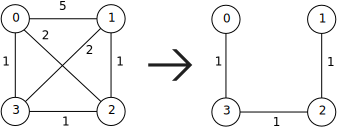
\includegraphics[width=0.75\textwidth,height=\textheight]{images/4.png}
\caption{Union by rank example}
\end{figure}

\begin{itemize}
\tightlist
\item
  \passthrough{\lstinline!arr[i]!} representation:

  \begin{itemize}
  \tightlist
  \item
    Case where \((\geq 0)\): parent of element of \(i\)
  \item
    Case where \((< 0)\): element \(i\) is the root of the tree and the
    size of the tree is \passthrough{\lstinline!abs(arr[i])!}
  \end{itemize}
\end{itemize}

\begin{figure}
\centering
\includegraphics[width=0.5\textwidth,height=\textheight]{images/5.png}
\caption{The forest formed by union-by-size, with the sizes encoded as
negative numbers}
\end{figure}

\hypertarget{practice-three}{%
\subsection{Practice Three}\label{practice-three}}

\begin{itemize}
\item
  Start with 10 one-element sets (so 10 single-node trees)

  \begin{longtable}[]{cccccccccc}
  \toprule
  \(0\) & \(1\) & \(2\) & \(3\) & \(4\) & \(5\) & \(6\) & \(7\) & \(8\)
  & \(9\)\tabularnewline
  \midrule
  \endhead
  \(-1\) & \(-1\) & \(-1\) & \(-1\) & \(-1\) & \(-1\) & \(-1\) & \(-1\)
  & \(-1\) & \(-1\)\tabularnewline
  \bottomrule
  \end{longtable}
\item
  Using union-by-size, try union\((1, 2)\), union\((3, 1)\),
  union\((5, 2)\), and union\((6, 3)\)
\item
  Draw the trees and fill the table
\end{itemize}

\hypertarget{complexity-revisited}{%
\subsection{Complexity Revisited}\label{complexity-revisited}}

\begin{itemize}
\tightlist
\item
  Worst case scenarios with \(n\) initial sets
\end{itemize}

\begin{longtable}[]{ccc}
\toprule
Approach & Union & Find\tabularnewline
\midrule
\endhead
Set of sets & \(O(n)\) & \(O(n)\)\tabularnewline
Quick find & \(O(n)\) & \(O(1)\)\tabularnewline
Tree (naive) & \(O(n)^*\) & \(O(n)\)\tabularnewline
Tree (rank union and naive find) & \(O(\log(n))^*\) &
\(O(\log(n))\)\tabularnewline
\bottomrule
\end{longtable}

\begin{itemize}
\tightlist
\item
  \(^*\): includes time to find the root; it's \(O(1)\) if the roots are
  given
\end{itemize}

\end{document}
